\documentclass[english,aspectratio=1610]{beamer} % Presentation mode
\usepackage[utf8]{inputenc}
\usepackage{cancel}

\usetheme{UUITmini} %Needs beamerthemeUUITmini.sty and UU_logo.eps/pdf.



\newcommand{\trnsp}{\mathsf{T}}

\newcommand{\mytitle}{Surprises in High-Dimensional Least Squares Interpolation}
\title[High-Dimensional Least Squares]{\mytitle}
\author{Ant\^{o}nio Horta Ribeiro}
\institute{Uppsala University}

\setbeamerfont{alerted text}{series=\bfseries}

\AtBeginSection[]{
	\begin{frame}
	\vfill
	\centering
			\usebeamerfont{title}\insertsectionhead\par%
	\vfill
\end{frame}
}

\date{}
\email{}  %Defined and used in UUITmini beamer theme


%Header and footer contents on all slides
%Examples of predefined strings to use: \insertshorttitle \insertsection \insertshortdate
\leftHead{}  %Empty is the default.
\rightHead{} %Empty is the default. 
\leftFoot{\insertemail} %\insertemail is the default
\rightFoot{\insertshorttitle} %\insertinstitute is the default

\begin{document}

\begin{frame}{}
	\vspace{-2mm}
	\begin{center}
		\begin{Large}
			\bfseries
		    Seminars: Overparametrized Machine Learning \\[2mm]
		\end{Large}
		\emph{\mytitle}
	\end{center}
	\vspace{-6mm}
	
	\begin{columns}[c]
		\begin{column}{50mm}
			\centering
			
			\vspace{8mm}
			
			\hspace*{4mm}    
\includegraphics[width=30mm]{uu_logo}
			
		\end{column}
		\begin{column}{65mm}
			\vspace{10mm}
			
			\textbf{Antônio Horta Ribeiro} \\
			\begin{small}
			    Dave Zacharias \\
			    Per Mattersson
			\end{small}
			
			\vspace{8mm}
			Division of Systems and Control \\
			Department of Information Technology
			Uppsala University \\
			\vspace{5mm}
			{\footnotesize
			it-seminar-overparameterized-ml@lists.uu.se}
		
			
			\par
			\vspace{0.8em}
			
		\end{column}
	\end{columns}
\end{frame}


\begin{frame}{Next seminar}
\begin{center}
	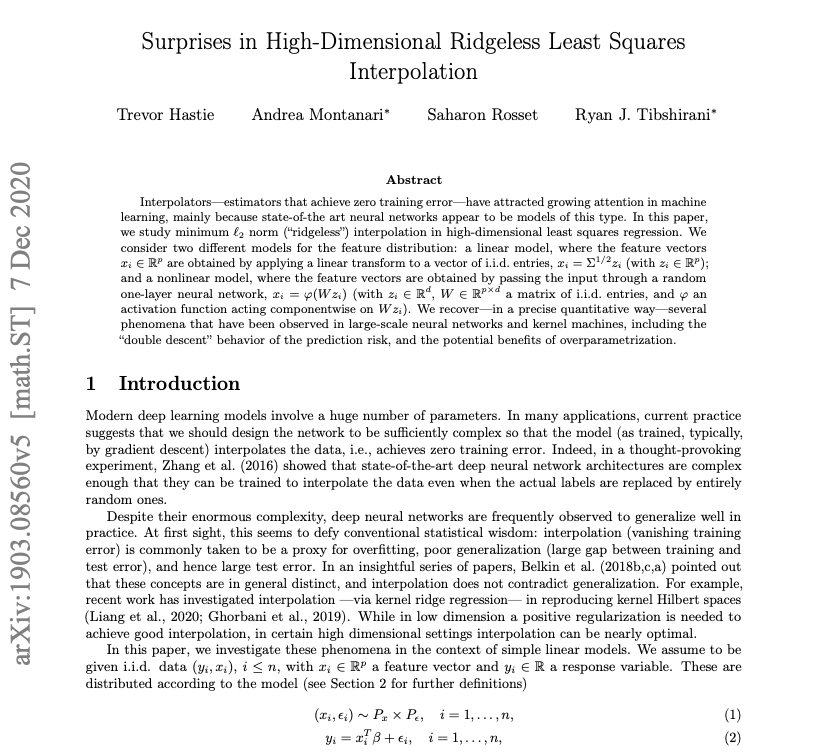
\includegraphics[width=.6\linewidth]{figures/paper.png}
\end{center}
\end{frame}

\section{Highlights}

\begin{frame}{Connection to neural networks (Section 1.2)}
\begin{itemize}
\item Let $\theta \in \mathbb{R}^m$ be the parameter vector.
\item $\theta  = \theta_0 + \beta$:
\item The number of parameters is so large that training effectively only changes the parameter by a small amount. Them $\beta$ is small and:

\begin{equation*}
\only<1>{
f(z; \theta) \approx  f(z; \theta_0) + \nabla_\theta f(z; \theta_0)^\trnsp\beta,}
\only<2>{
f(z; \theta) \approx  \cancelto{}{f(z; \theta_0)} + \overbrace{\nabla_\theta f(z; \theta_0)^\trnsp}^{x^\trnsp}\beta,}
\end{equation*}

\end{itemize}

\tiny{Chizat, L., Oyallon, E., and Bach, F. \textit{On {Lazy} {Training} in {Differentiable} {Programming}.} Neural Information Processing Systems (NeurIPS), 2019}	\\	

\end{frame}

\begin{frame}{Connection to neural networks (Section 1.2)}
\begin{itemize}
\item
Nonlinear map to feature space: $z \mapsto \nabla_\theta f(z; \theta_0) = x$
\item Regression on the feature space:
\begin{equation*}
y = x^\trnsp \beta
\end{equation*}

\item More about that line in Seminar S4:
\vspace{13pt}

\tiny{Jacot, A., Gabriel, F., and Hongler, C. \textit{Neural {Tangent} {Kernel}: {Convergence} and {Generalization} in
  {Neural} {Networks}.} Neural Information Processing Systems (NeurIPS), 2018}	

\end{itemize}
\end{frame}

\begin{frame}{Ridgeless least squares  (Section 2.2)}

\textbf{Estimated parameter:} using train dataset $(\textcolor{red}{x_t}, \textcolor{blue}{y_t})$, $t = 1, \cdots, n$:
\begin{itemize}
    \item<2-> Underparametrized:
    \begin{equation*}
       \min_{\textcolor{cyan}{\theta}} \sum_t (\textcolor{blue}{y_i} - \textcolor{cyan}{\theta}^\trnsp \textcolor{red}{x_t})^2
    \end{equation*}
    \item<3> Overparametrized:
        \begin{equation*}
        \begin{aligned}
            \min_{\textcolor{cyan}{\theta}} & \|\textcolor{cyan}{\theta}\|_2^2\\
             \text{subject to }& \textcolor{blue}{y_t} = \textcolor{cyan}{\theta}^\trnsp \textcolor{red}{x_t} \\
            & \text{for every } t = 1, \cdots, n
        \end{aligned}
    \end{equation*}
    \item<3> Connection with gradient descent (\textit{Proposition 1}). \\
    \scriptsize{ See also:
    \href{https://math.stackexchange.com/q/3499305}{https://math.stackexchange.com/q/3499305}}
\end{itemize}

\end{frame}


\begin{frame}{Isotropic features (Section 3)}
    \begin{center}
	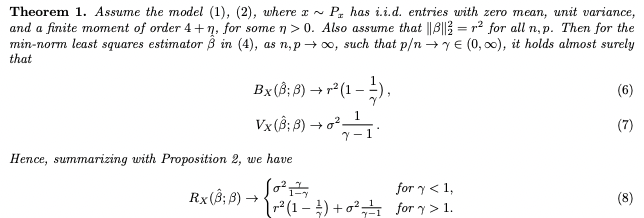
\includegraphics[width=.8\linewidth]{figures/thm1.png}
    \end{center}
\end{frame}

\begin{frame}{Isotropic features (Section 3)}
    \begin{center}
	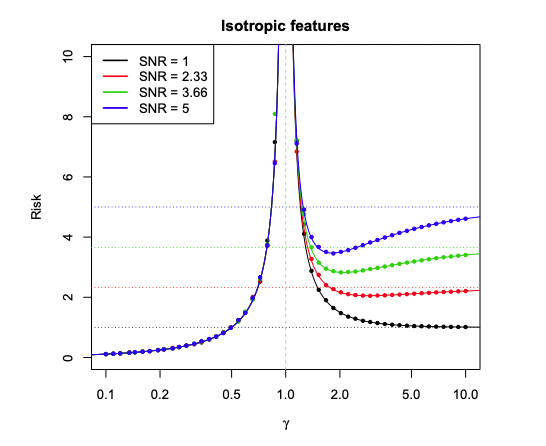
\includegraphics[width=.6\linewidth]{figures/fig1.png}
    \end{center}
\end{frame}

\begin{frame}{}
\begin{center}
\begin{block}{NOTE!}
        We will only cover sections 1, 2 and 3 of this paper (first 11 pages)!
\end{block}        
\end{center}
\end{frame}

\section{Background}

\begin{frame}{Wigner matrix and semicircle distribution}

\begin{columns}[c]
	\begin{column}{70mm}
\begin{itemize}
\item 
Assume a symmetric matrix: ($W \sim W^\trnsp$)
\begin{equation*}
   W = 
    \begin{bmatrix}
        w_{1, 1} & w_{1, 2} & w_{1, 3}\\
        w_{2, 1} & w_{2, 2} & w_{2, 3}\\
        w_{3, 1} & w_{3, 2} & w_{3, 3}
    \end{bmatrix}
\end{equation*}

with the lower diagonal entries i.i.d. sampled from a random distribution. 
\item What can be said about the eigenvalues of such a matrix.

    \item The idea was introduced by Eugene Wigner when working with heavy nuclei atoms.\\
\vspace{10pt}
\tiny{E. P. Wigner. Characteristic vectors of bordered matrices with infinite dimensions.
Annals Math., 62:548–564, 1955.}
\end{itemize}
\end{column}
	\begin{column}{53mm}
	Distribution of eigenvalues.
	    \begin{center}
	        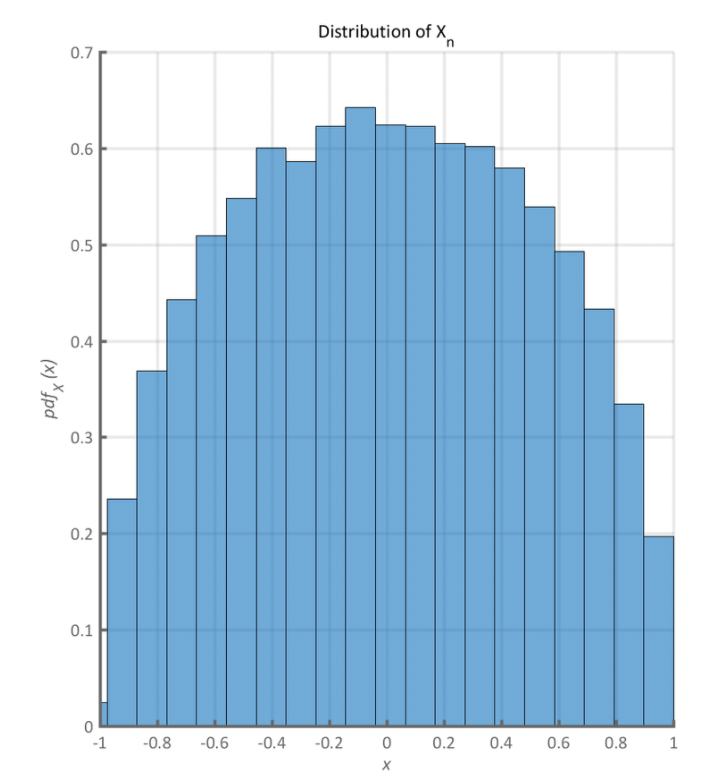
\includegraphics[width=.9\linewidth]{figures/wigner.png}
            \tiny{Wigner PDF (Kris Buchanan). License: CC BY-SA 4.0.}
            \tiny{\texttt{en.wikipedia.org/wiki/Wigner\_semicircle\_distribution}}
        \end{center}
	\end{column}
\end{columns}
\end{frame}

\begin{frame}{Wishart matrix and the Marchenko–Pastur distribution}
	\begin{itemize}
    \item 
    Let now A be
    \begin{equation*}
       A = 
        \begin{bmatrix}
            a_{1, 1} & a_{1, 2} & a_{1, 3}\\
            a_{2, 1} & a_{2, 2} & a_{2, 3}
        \end{bmatrix}
    \end{equation*}
    with the lower diagonal entries i.i.d. sampled from a random distribution. 
     \item 
     What is the distribution of the eigen values of:
     \begin{equation*}
     A^\trnsp A ?
    \end{equation*}
    \end{itemize}
    \begin{center}
	        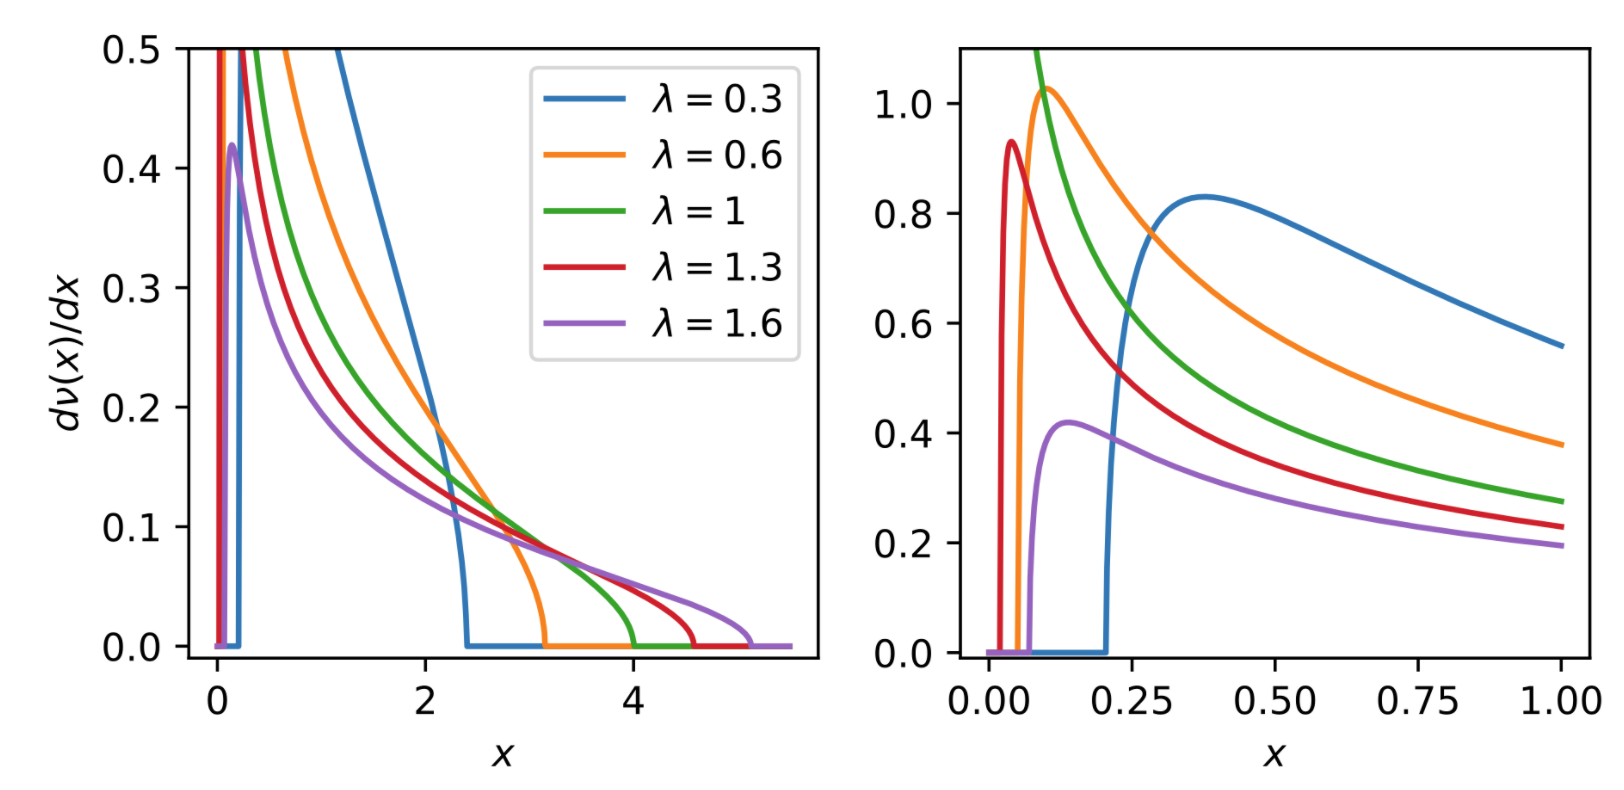
\includegraphics[width=.5\linewidth]{figures/mp distribution.png}\\
            \tiny{Marchenko-Pastur distribution  (Mario Geiger). License: CC BY-SA 4.0.}\\
            \tiny{\texttt{en.wikipedia.org/wiki/Marchenko–Pastur\_distribution}}
            
        \end{center}
\end{frame}



\begin{frame}{Random matrix theory}
References:

\vspace{10pt}
\begin{itemize}\tiny{
    \item G.~W. Anderson, A.~Guionnet, and O.~Zeitouni.
\emph{An {Introduction} to {Random} {Matrices}}, 2009.}\\
 \item \tiny{Z.~Bai and J.~W. Silverstein.
\emph{Spectral analysis of large dimensional random matrices},
  volume~20 of \emph{Springer {Series} in {Statistics}}.
Springer, 2010}
\item \tiny{T.~Tao. \emph{Topics in random matrix theory}, volume 132 of \emph{Graduate
  {Studies} in {Mathematics}}. American Mathematical Society, 2012.}
\end{itemize}

\vspace{20pt}

Other sources:


\vspace{10pt}
\begin{itemize}\tiny{
    \item ICML 2021 tutorial: https://random-matrix-learning.github.io/}
\end{itemize}

\end{frame}

\end{document}
